% Options for packages loaded elsewhere
\PassOptionsToPackage{unicode}{hyperref}
\PassOptionsToPackage{hyphens}{url}
%
\documentclass[
]{article}
\usepackage{changepage}
\usepackage{amsmath,amssymb}
\usepackage{lmodern}
\usepackage{iftex}

\usepackage{booktabs}
\usepackage{ragged2e}
\usepackage{graphicx}
% Decrease margin spacing
\usepackage[margin=1in]{geometry}
\ifPDFTeX
  \usepackage[T1]{fontenc}
  \usepackage[utf8]{inputenc}
  \usepackage{textcomp} % provide euro and other symbols
\else % if luatex or xetex
  \usepackage{unicode-math}
  \defaultfontfeatures{Scale=MatchLowercase}
  \defaultfontfeatures[\rmfamily]{Ligatures=TeX,Scale=1}
\fi
% Use upquote if available, for straight quotes in verbatim environments
\IfFileExists{upquote.sty}{\usepackage{upquote}}{}
\IfFileExists{microtype.sty}{% use microtype if available
  \usepackage[]{microtype}
  \UseMicrotypeSet[protrusion]{basicmath} % disable protrusion for tt fonts
}{}
\makeatletter
\@ifundefined{KOMAClassName}{% if non-KOMA class
  \IfFileExists{parskip.sty}{%
    \usepackage{parskip}
  }{% else
    \setlength{\parindent}{0pt}
    \setlength{\parskip}{6pt plus 2pt minus 1pt}}
}{% if KOMA class
  \KOMAoptions{parskip=half}}
\makeatother
\usepackage{xcolor}
\usepackage{longtable,booktabs,array}
\usepackage{calc} % for calculating minipage widths
% Correct order of tables after \paragraph or \subparagraph
\usepackage{etoolbox}
\makeatletter
\patchcmd\longtable{\par}{\if@noskipsec\mbox{}\fi\par}{}{}
\makeatother
% Allow footnotes in longtable head/foot
\IfFileExists{footnotehyper.sty}{\usepackage{footnotehyper}}{\usepackage{footnote}}
\makesavenoteenv{longtable}
\setlength{\emergencystretch}{3em} % prevent overfull lines
\providecommand{\tightlist}{%
  \setlength{\itemsep}{0pt}\setlength{\parskip}{0pt}}
\setcounter{secnumdepth}{-\maxdimen} % remove section numbering
\ifLuaTeX
  \usepackage{selnolig}  % disable illegal ligatures
\fi
\IfFileExists{bookmark.sty}{\usepackage{bookmark}}{\usepackage{hyperref}}
\IfFileExists{xurl.sty}{\usepackage{xurl}}{} % add URL line breaks if available
\urlstyle{same} % disable monospaced font for URLs
\hypersetup{
  hidelinks,
  pdfcreator={LaTeX via pandoc}}

\author{}
\date{}

\begin{document}
\justify

\begin{center}
{\Large \textbf{Levy Flight based FOX optimizer}}\\
\end{center}


\begin{center}
{\fontsize{10}{14}\selectfont \textbf{Sanya Garg, Tripti Gusain, Himanshi}}
\end{center}

\begin{center}
\emph{Netaji Subhas University of Technology}\\
\vspace{3em} % Adjust the vertical space as needed
\hrule
\end{center}

\vspace{1em} 
\begin{justify}
\textbf{Abstract}

\noindent
Optimization algorithms play a crucial role in solving complex problems across various domains. The FOX algorithm is a recently proposed metaheuristic optimization technique that exhibits promising performance in complex real-life problems. In this paper, we propose a modification to the FOX algorithm by integrating Levy flight, a stochastic search strategy known for its ability to efficiently explore large solution spaces. The modified FOX algorithm, termed LFFO, combines the exploitation capabilities of the FOX algorithm with the exploration capabilities of Levy flight to enhance its search capabilities and convergence speed. We conduct extensive experiments on a set of benchmark functions to evaluate the performance of LFFO against other state-of-the-art optimization algorithms. The results demonstrate that LFFO exhibits superior exploration and exploitation abilities, leading to improved convergence rates and higher-quality solutions compared to the original FOX algorithm and several benchmark algorithms. Our findings highlight the effectiveness of incorporating Levy flight into metaheuristic optimization algorithms like FOX, showcasing its potential for addressing challenging optimization problems in real-world applications.

\noindent
\begin{justify}
\textbf{Keywords:}\\
FOX Optimizer . Levy Flight . Benchmark test functions . Pressure vessel design problem . Piston Lever
\end{justify}

\vspace{1.5em} 
\hrule

\vspace{0.5em} 
\def\labelenumi{\arabic{enumi}.}
\item
\vspace{5mm}
  \textbf{1. Introduction}

In recent years, nature-inspired metaheuristic algorithms have garnered considerable attention for their efficacy in solving complex optimization problems across diverse domains. Among these algorithms, the Fox-inspired Optimization Algorithm (FOA) has emerged as a promising solution. However, like many metaheuristic algorithms, the original FOA may encounter issues such as slow convergence and stagnation in local optima.

To address these challenges and enhance FOA's performance, recent research efforts have explored integrating innovative techniques from other metaheuristic algorithms. One such notable advancement is the introduction of the Levy flight-based Grasshopper Optimization Algorithm (GOA), proposed by Lei Wu, Jiawei Wu, and Tengbin Wang (2023). This novel approach incorporates Levy flight strategies into the GOA framework, resulting in improved exploration capabilities and convergence behavior. Inspired by the success of Levy flight-based GOA, this paper extends these principles to the Fox Algorithm framework.

By embedding Levy flight strategies into the Fox Algorithm, search capabilities are enhanced and limitations such as slow convergence and local optima stagnation are overcomed. This paper builds upon the strengths of both the Fox Algorithm and Levy flight mechanisms, creating a more robust and efficient optimization framework.

The subsequent sections of this paper provide a detailed overview of the integrated Levy flight-based Fox Optimization Algorithm (LFFOA). The methodology is discussed, and the algorithm's pseudo-code is presented, along with an evaluation of its performance through extensive experimentation. Furthermore, LFFOA's application in solving real-world optimization problems is showcased, leveraging analyses from CEC2014 and CEC2017 benchmark functions to validate its effectiveness.

Additionally, a comprehensive methodological approach is employed to thoroughly evaluate the performance and significance of the LFFOA. Through rigorous statistical analysis, including the application of the Wilcoxon ranksum test for significance analysis, the superiority of LFFOA over other heuristic algorithms is demonstrated. This comprehensive approach ensures a rigorous evaluation and validation of the LFFOA, elucidating its effectiveness in solving optimization problems across various domains.

The study concludes that the integration of Levy flight strategies into the Fox Algorithm framework significantly enhances its performance and robustness, making LFFOA a compelling choice for addressing optimization challenges across diverse domains.

\def\labelenumi{\arabic{enumi}.}
\item
\vspace{5mm}
  \textbf{2. Basic Fox-inspired Optimization Algorithm}

The Fox Optimization Algorithm (FOX) initiates by initializing a population represented by the \(X\) matrix, where each row corresponds to the position of red foxes. Subsequently, the fitness of each search agent (row) in the \(X\) matrix is calculated using standard benchmark functions. Throughout iterations, FOX tracks the \(BestFitness\) and \(BestX\) by comparing the fitness values of search agents.

To balance exploration and exploitation phases, FOX employs a condition with a random variable, allocating 50\% probability to each phase in each iteration. This ensures that nearly half of the iterations are dedicated to exploration and the remaining half to exploitation. The algorithm utilizes a variable, denoted as \(a\) to adjust search performance based on the \(BestX\) value. Moreover, the fitness value plays a crucial role in guiding search agents to avoid local optima. If a new position does not yield a change in fitness, the exploration phase is deactivated to allow other phases to take effect. Overall, FOX's iterative process and strategic adjustments facilitate effective exploration and exploitation, preventing the algorithm from getting trapped in local optima.

In the exploitation phase, FOX determines whether to find a new position for the red fox based on a random variable \(p\). If \(p\) exceeds 0.18, FOX calculates parameters such as the distance sound travels \(Dist\_S\_T_{\text{\textit{it}}}\)
 , the distance between the fox and its prey  \(Dist\_Fox\_Prey_{\text{\textit{it}}}\), and the jumping value \(Jump_{\text{\textit{it}}}\) . Additionally, a random number within [0,1] is generated to compute the sound travel time \(Time\_S\_T_{\text{\textit{it}}}\). The distance traveled by the sound is determined by multiplying the speed of sound in the air \(Sp\_S\) with the sound travel time.

\[
Dist\_S\_T_{\text{\textit{it}}} = Sp\_S \times Time\_S\_T_{\text{\textit{it}}} \tag{1}
\]


The time taken for sound to travel between a fox and its prey, represented by the variable \(Time\_S\_T_{\text{\textit{it}}}\) which is a random number in the range [0, 1]. Additionally, another equation is introduced to determine  \(Sp\_S\) which represents the speed of sound based on the best position found so far, denoted by \(BestPosition_{\text{\textit{it}}}\) where \(it\) refers to the iteration. Equation (2) outlines the method for calculating \(Sp\_S\) using the best position.

\[
(Sp\_S) = \frac{BestPosition_{\text{\textit{it}}}}{Time\_S\_T_{\text{\textit{it}}}} \tag{2}
\]

The distance traveled by sound is halved to determine the distance between the fox and the prey . This is because the sensor sends a sound wave signal to the object and receives it back, effectively doubling the distance traveled by the sound wave. Equation (3) represents this concept.

\[
(Dist\_Fox\_Prey_{\text{\textit{it}}}) = (Dist\_S\_T_{\text{\textit{it}}}) \times 0.5 \tag{3}
\]


After finding the distance between a fox and the prey, the red fox needs to find a new position so that the red fox requires to jump to catch the prey. Therefore, the fox needs to calculate the jump height \(Jump_{\text{\textit{it}}}\). Thus, \(Jump_{\text{\textit{it}}}\) can be calculated by the following equation:

\[
(Jump_{\text{\textit{it}}}) = 0.5 \times 9.81 \times t^2 \tag{4}
\]


Then, the Jump value is multiplied by \(Dist\_Fox\_Prey_{\text{\textit{it}}}\) and \(c_{\text{\textit{1}}}\). The variable \(c_{\text{\textit{1}}}\) has a range, which is within [0, 0.18] when the red fox jumps to the northeast direction. Calculation of the new position of the red fox if the \( p\), which random number in the range [0,1], is greater than 0.18 is shown in equation (5)

\[
X_{\text{\textit{it+1}}} = Dist\_Fox\_Prey_{\text{\textit{it}}} \times Jump_{\text{\textit{it}}} \times c_{\text{\textit{1}}} \tag{5}
\]


If p is greater than 0.18, then the new position is calculated by Eq. (5). However, if the value is less than 0.18, then the new position is calculated by equation (6). The range of \(c_{\text{\textit{1}}}\) is within [0.19, 1].

\[
X_{\text{\textit{it+1}}} = Dist\_Fox\_Prey_{\text{\textit{it}}} \times Jump_{\text{\textit{it}}} \times c_{\text{\textit{2}}} \tag{6}
\]

The value of \(c_{\text{\textit{1}}}\) and \(c_{\text{\textit{2}}}\) are 0.18 and 0.82 respectively. These values are based on the jump movement of a red fox, which is either jumps to the northeast or opposite. Therefore, if the \(p\) value is greater than 0.18, it means that the red fox jumps to the northeast direction


During the exploitation phase, to control the random walk, the fox searches randomly in this phase according to the best position of the fox that has been found so far. The fox does not have a jumping technique in this phase because it has to walk randomly to explore prey in the search area. To ensure that the fox walks randomly toward the best position, a minimum time variable \(MinT\) and the variable a are used to control the search. Equations (7) and (8) show the calculation of the \(MinT\) and variables. \(MinT\) is calculated by finding the minimum of \(tt\).

\begin{equation}
tt = \frac{\sum (Time_{S_T_{\text{\textit{it}}}} (i,:))}{\text{dimension}}, \quad MinT = \Min(tt) \tag{7}
\end{equation}


Summation of \(Time_{S_T_{\text{\textit{it}}}} (i,:)\)  is divided on the dimension of the problem to find the minimum time average \(tt\) where \(Max_{\text{\textit{it}}}\), is the maximum iterations.

\begin{equation}
a = 2 \times \left[ 1 - \left( \frac{1}{\(Max_{\text{\textit{it}}}} \right) \right] \tag{8}
\end{equation}


Rand(1, dimension) is used to ensure that the fox walks stochastically to explore the prey. However, to strengthen the searchability of FOX both \(MinT\) and \(a\) variable are used.
Variable \(r\), which is a random number, is also used to balance the exploration and exploitation phases. Equation (9) shows the exploration technique of the fox in searching for a new position in the search space \(X_{\text{\textit{it+1}\)}.

\begin{equation}
X_{\text{\textit{it+1}}} = BestX_{\text{\textit{it}}} \times \text{rand}(1,\text{dimension}) \times \text{MinT} \times a \tag{9}
\end{equation}

\\\\\\\

\def\labelenumi{\arabic{enumi}.}
\item
\vspace{5mm}
  \textbf{3. Pseudocode of Fox Optimization Algorithm}

The pseudocode of FOA is given in Algorithm 1:

\begin{longtable}{@{}p{\dimexpr\linewidth-2\tabcolsep\relax}@{}}
\toprule
\begin{minipage}[b]{\linewidth}
\raggedright
\textbf{Algorithm 1: Fox Optimization Algorithm}
\end{minipage} \\
\midrule
\endhead
\begin{minipage}[t]{\linewidth}
\raggedright
\begin{enumerate}
  \item Initialize the red fox population $X$ \textit{i (i=1,2,....,n)}
  \item While $it < Maxit$
  \item \hspace{0.5cm} Initialize $Dist\_S\_T$, $Sp\_S$, $Time\_S\_T$, $BestX$, $Dist\_Fox\_Prey$, $Jump$, $MinT$, $a$, $BestFitness$
  \item \hspace{0.5cm} Calculate the fitness of each search agent
  \item \hspace{0.5cm} Select $BestX$ and $BestFitness$ among the fox population ($X$) in each iteration.
  \item \hspace{0.5cm} \textbf{If} $fitness_{\text{\textit{i}}} > fitness_{\text{\textit{i+1}}}$ 
  \item \hspace{1cm} $BestFitness = fitness_{\text{\textit{i+1}}}$
  \item \hspace{1cm} $BestX=X(i, :)$
  \item \hspace{0.5cm} \textbf{EndIf1}
  \item \hspace{0.5cm} \textbf{If2} $r \geq 0.5$ 
  \item \hspace{1cm} \textbf{If3} $p>0.18$ 
  \item \hspace{1.5cm} Initialize time randomly
  \item \hspace{1.5cm} Calculate $Distance\_Sound\_travels$ using Eq. (1)
  \item \hspace{1.5cm} Calculate $Sp\_S$ from Eq. (2)
  \item \hspace{1.5cm} Calculate distance from fox to prey using Eq. (3)
  \item \hspace{1.5cm} $Tt =$ average time
  \item \hspace{1.5cm} $T=Tt/2$
  \item \hspace{1.5cm} Calculate jump using Eq. (4)
  \item \hspace{1.5cm} Find $X_{\text{\textit{it+1}}}$ using Eq. (5)
  \item \hspace{1cm} \textbf{Elseif} $p \leq 0.18$ 
  \item \hspace{1.5cm} Initialize time randomly
  \item \hspace{1.5cm} Calculate $Distance\_Sound\_travels$ using Eq. (1)
  \item \hspace{1.5cm} Calculate $Sp\_S$ from Eq. (2)
  \item \hspace{1.5cm} Calculate distance from fox to prey using Eq. (3) 
  \item \hspace{1.5cm} $Tt =$ average time
  \item \hspace{1.5cm} $T=Tt/2$
  \item \hspace{1.5cm} Calculate jump using Eq. (4)
  \item \hspace{1.5cm} Find $X_{\text{\textit{it+1}}}$ using Eq. (6)
  \item \hspace{1cm} \textbf{EndIf3}
  \item \hspace{0.5cm} \textbf{Else}
  \item \hspace{1cm} Find $MinT$ using Eq. (7)
  \item \hspace{1cm} Explore $X_{\text{\textit{it+1}}}$ using Eq. (9)
  \item \hspace{0.5cm} \textbf{EndIf2}
  \item \hspace{0.5cm} Check and amend the position if it goes beyond the limits
  \item \hspace{0.5cm} Evaluate search agents by their fitness
  \item \hspace{0.5cm} Update $BestX$
  \item \hspace{0.5cm} $it=it+1$
  \item \textbf{EndWhile}
  \item return $BestX$ and $BestFitness$
\end{enumerate}
\end{minipage} \\
\bottomrule
\end{longtable}

\def\labelenumi{\arabic{enumi}.}
\item
\vspace{5mm}
  \textbf{4. Modifications}

The modified version of the Fox Optimization Algorithm introduces several significant adjustments aimed at enhancing its performance and efficiency in solving optimization problems.

\textbf{Mantegna’s algorithm from levy flights random walks}

Study shows that the distribution probability density function of the variation of the Levy’s flight step can be approximated as follows:

\begin{equation}
L(s) \sim |s|^{-1 - \theta} \tag{10}
\end{equation}

Where s is the random step length of Levy’s flight behavior, and 
 is bounded as [0, 2] as a power-law index and is set to be 1.5, which controls the peak sharpness of the levy distribution graph. The different values of the parameter 
 cause different distributions, it makes longer jumps for smaller values, whereas it makes shorter jumps for bigger values. True Levy distribution is hard to implement in computer code, but the approximate form. Mantegna algorithm is one of the fast and accurate algorithms which generate a stochastic variable whose probability density is close to the Levy stable distribution characterized. Mantegna’s algorithm can be split into three steps. For random walks, Mantegna’s algorithm determines the step length S as follows:

\begin{equation}
S = \frac{U}{|V|^\frac{1}{\theta}} \tag{11}
\end{equation}

where S is the random step length variable, while U and V are two normal stochastic variables with standard deviation \(\sigma _U\)
 and \(\sigma _V\)
, U and V should be attained based on normal distributions:

\begin{equation}
U \sim N\left(0, \sigma_U^2\right), \quad V \sim \left(0, \sigma_V^2\right) \tag{12}
\end{equation}

The symbol \(\sim\)
 in Eq. (12) denotes that the random variable obeys the distribution on the right-hand side; that is, samples should be drawn from the distribution. As the standard deviation \(\sigma _U\)
 and \(\sigma _V\)
 cannot be chosen independently for an arbitrary value of 
, for simplicity we usually set

\begin{equation}
\sigma_V = 1 \tag{13}
\end{equation}

After this setting, the standard deviation 
 can be obtained by:

\begin{equation}
\sigma_{U} = \left\{ \frac{\Gamma(1 + \theta) \times \sin(0.5\pi \theta)}{\Gamma\left[0.5\left(1 + \theta\right)\right]\times \theta \times 2^{0.5(\theta - 1)}} \right\}^{\frac{1}{\theta}} \tag{14}
\end{equation}

The step size of Levy flight has been achieved by the Eqs. (10) – (14), which simulate the search of short walking distance and occasionally longer walking distance. Then the step size is calculated by

\begin{equation}
\text{\textit{step size}} = f \times S \tag{15}
\end{equation}

Where, the factor value\( f(f=0.01)\)
 derived from \(L\)/100 determines the levy walks and the factor is dependent on the dimension of the desired problem, where \(L\) is the wide-scale; unless Levy flights become too aggressive, it helps the new solution move away from the search space. The process of Levy flight can be exhibited in Algorithm 1.

\begin{longtable}{@{}p{\dimexpr\linewidth-2\tabcolsep\relax}@{}}
\toprule
\begin{minipage}[b]{\linewidth}
\raggedright
\textbf{Algorithm 2: Levy Flight}
\end{minipage} \\
\midrule
\endhead
\begin{minipage}[t]{\linewidth}
\raggedright
\begin{enumerate}
  \item \textbf{Require:} Current Position
  \item \textbf{Ensure:} New Position
  \item Calculate the step length S based on Mantegna algorithm using Eq. (11)
  \item $S = \frac{U}{|V|^\frac{1}{\theta}}$
  \item $U$ and $V$ based on normal distributions are gained by Eq. (12)
  \item $U \sim N\left(0, \sigma_U^2\right), \quad V \sim \left(0, \sigma_V^2\right)$
  \item For simplicity, set $\sigma_V$ = 1
  \item Calculate $\sigma_U$ using Eq. (14)
  \item Calculate step size using Eq. (15) 
  \item $\text{\textit{step size}} = f \times S$
  \item Execute the actual random walk or flight with:
  \item $levy\_step = \sigma \cdot randn(1, dim) / (rand()^{(1 / \beta)})$
  \item $Best\_pos = BestX + levy\_step$
  \item return $Best\_pos$
  \item End
\end{enumerate}
\end{minipage} \\
\bottomrule
\end{longtable}


The step size value will be added to update the equations of the LFFOA algorithm for finding the best position. From theoretical perspectives, this random walk is based on a long tail distribution which can be used to help an algorithm escape from getting stuck at a local optimum. In other words, the Levy flight distribution is an effective mathematical operator for producing varied solutions in the searching space and increasing the exploration capability of the LFFOA algorithm.

Firstly, $levy\_step = \sigma \cdot randn(1, dim) / (rand()^{(1 / \beta)})$
 represents the Levy flight function, and dim is the dimension size of the problem. the Levy flight Strategy is integrated into the FOA by the above formula. The Levy flight has a relatively high probability of large strides in random walking, which can effectively improve the randomness of the FOA algorithm. This way, the risk that the algorithm gets stuck in a local optimum is drastically reduced, while it is still possible to perform sufficient local refinements. In other words, the algorithm presents a natural balance between exploration and exploitation.

Secondly, in the case of stagnation, Levy-triggered searching (hunting) patterns can help LFFOA to jump out of them toward new better positions. By this mechanism, the LFFOA algorithm can overcome the deficiencies of the little diversity of the origin FOA algorithm and greatly increase the probability of getting the best position (solution), which is also the highlight and unique feature of the LFFOA algorithm.

Despite being a simple change in the FOA algorithm, this new distribution induces drastic changes in the optimization process, LFFOA-based jumps can redistribute foxes around the fitness landscape to prevent the population from the loss of diversity and to put more emphasis on the global searching tendency.

\newpage
\begin{minipage}[t]{\textwidth}
  \textbf{5. Pseudocode of Modified Fox Optimization Algorithm}
  
  \begin{longtable}{@{}p{\dimexpr\linewidth-2\tabcolsep\relax}@{}}
  \toprule
  \begin{minipage}[b]{\linewidth}
  \raggedright
  \textbf{Algorithm 2 : Modified Fox Optimization Algorithm}
  \end{minipage} \\
  \midrule
  \endhead
  \begin{minipage}[t]{\linewidth}
  \raggedright
  \begin{enumerate}
    \item Initialize the red fox population $X_i$ ($i=1, 2, ...n$)
    \item Add the parameters for Levy Flight:
      \begin{itemize}
        \item $\beta = 1.5$ (scaling parameter for Levy flight)
        \item Calculate $\sigma$
      \end{itemize}
    \item While $it < Maxit$
    \item \hspace{0.5cm} Initialize $Dist\_S\_T$, $Sp\_S$, $Time\_S\_T$, $BestX$, $Dist\_Fox\_Prey$, $Jump$, $MinT$, $a$, $BestFitness$
    \item \hspace{0.5cm} Calculate the fitness of each search agent
    \item \hspace{0.5cm} Select $BestX$ and $BestFitness$ among the fox population ($X$) in each iteration.
   \item \hspace{0.5cm} \textbf{If} $fitness_{\text{\textit{i}}} > fitness_{\text{\textit{i+1}}}$ 
  \item \hspace{1cm} $BestFitness = fitness_{\text{\textit{i+1}}}$
  \item \hspace{1cm} $BestX=X(i, :)$
  \item \hspace{0.5cm} \textbf{EndIf1}
  \item \hspace{0.5cm} \textbf{If2} $r \geq 0.5$ 
  \item \hspace{1cm} \textbf{If3} $p>0.18$ 
  \item \hspace{1.5cm} Initialize time randomly
  \item \hspace{1.5cm} Calculate $Distance\_Sound\_travels$ using Eq. (1)
  \item \hspace{1.5cm} Calculate $Sp\_S$ from Eq. (2)
  \item \hspace{1.5cm} Calculate distance from fox to prey using Eq. (3)
  \item \hspace{1.5cm} $Tt =$ average time
  \item \hspace{1.5cm} $T=Tt/2$
  \item \hspace{1.5cm} Calculate jump using Eq. (4)
  \item \hspace{1.5cm} Find $X_{\text{\textit{it+1}}}$ using Eq. (5)
  \item \hspace{1cm} \textbf{Elseif} $p \leq 0.18$ 
  \item \hspace{1.5cm} Initialize time randomly
  \item \hspace{1.5cm} Calculate $Distance\_Sound\_travels$ using Eq. (1)
  \item \hspace{1.5cm} Calculate $Sp\_S$ from Eq. (2)
  \item \hspace{1.5cm} Calculate distance from fox to prey using Eq. (3) 
  \item \hspace{1.5cm} $Tt =$ average time
  \item \hspace{1.5cm} $T=Tt/2$
  \item \hspace{1.5cm} Calculate jump using Eq. (4)
  \item \hspace{1.5cm} Find $X_{\text{\textit{it+1}}}$ using Eq. (6)
  \item \hspace{1cm} \textbf{EndIf3}
    \item \hspace{0.5cm} \textbf{Else}
    \item \hspace{1cm} Find $MinT$ using Eq. (7)
    \item \hspace{1cm} Explore $X(it+1)$ using Eq. (9)
    \item \hspace{1cm} Explore new positions using Levy Flight:
    \item \hspace{1.5cm} $levy\_step = \sigma \cdot randn(1, dim) / (rand()^{(1 / \beta)})$
    \item \hspace{1.5cm} $ans(i, :) = Best\_pos + levy\_step$ 
    \item \hspace{0.5cm} \textbf{EndIf}
    \item \hspace{0.5cm} Check and amend the position if it goes beyond the limits
    \item \hspace{0.5cm} Evaluate search agents by their fitness
    \item \hspace{0.5cm} Update $BestX$
    \item \hspace{0.5cm} $it=it+1$
    \item \textbf{EndWhile}
  \end{enumerate}
  \end{minipage} \\
  \bottomrule
  \end{longtable}
\end{minipage}
\newpage

\def\labelenumi{\arabic{enumi}.}
\item
\vspace{5mm}
  \textbf{6. Results and Discussions}

To ensure that the modified algorithm works well, it must be tested by using different benchmark test functions.The performance evaluation of the modified FOX algorithm includes the utilization of benchmark functions from CEC2017 and CEC2014. These benchmark functions serve as critical metrics to assess the efficacy of the proposed modifications. Besides, the results of the modified algorithm are compared to SCSO, AOA, GWO, COA, SHO, ChOA, PDO and FOX. Then, Wilcoxon rank-sum test is employed to determine the statistical significance of the modification. 

\def\labelenumi{\arabic{enumi}.}
\item
\vspace{5mm}
  \textbf{6.1.1 CEC2014 benchmark test functions}
  
  The CEC2014 benchmark functions suite comprises a diverse set of optimization problems designed to assess the performance of optimization algorithms. Developed as part of the IEEE Congress on Evolutionary Computation in 2014, these functions mimic real-world optimization challenges, including multimodality, nonlinearity, and high dimensionality. By providing standardized benchmarks, the suite facilitates rigorous evaluation and comparison of optimization algorithms, aiding advancements in evolutionary computation and optimization research.

  The FOX\_Levy is compared with SCSO, AOA, GWO, COA, SHO, ChOA, PDO and FOX.
This search is performed using 2000 iterations.The results are determined after running each algorithm 50 times, and then the average/mean results are used for comparison. In our evaluation spanning 30 functions, FOX\_Levy excels, outperforming other algorithms in 6 instances, while FOX leads in 3 cases. GWO demonstrates the most consistent superiority, prevailing in 8 functions, followed by SHO in 3. Both COA and SCSO show promise in 1 function each. FOX\_Levy also achieves top results alongside other algorithms in 8 functions. Conversely, PDO, AOA and ChOA consistently perform poorly across all functions. GWO emerges as the most reliable performer across the majority of functions.

\begin{table}[h!]
\caption{Comparision based on mean}
\scriptsize % Reduce font size
\begin{tabular}{||c c c c c c c c c c||}
\hline
F & SCSO  & AOA & GWO & COA & SHO & ChOA & FOX & FOX-LEVY & PDO\\ [1ex]
\hline\hline
1 & 7.17E+06 & 1.80E+07 & 6.36E+06 & 1.04E+08& 8.69E+06& 1.29E+07& 1.02E+05& 2.27E+05 &70241547.14\\ 
2 & 8.79E+07 & 3.72E+09 & 1.33E+06 & 4.99E+09& 5.18E+08& 2.37E+09& 853.2552& 4.73E+05 &3413182438\\ 
3 & 4.66E+03 & 1.85E+04 & 5.65E+03 & 1.19E+04& 3.80E+03& 1.90E+04& 1.72E+04& 2.71E+03 & 12789.2239 \\ 
4 & 434.0312 & 966.8375 & 433.8592 & 1.98E+03& 457.2668& 566.3132& 428.047& 428.028 & 944.1082037 \\
5 & 520.0912 & 520.078 & 520.0735 & 520.3763& 519.999& 520.4265& 521.0001& 520.449 & 520.2025416 \\
6 & 605.2975 & 609.3803 & 602.144 & 609.931& 605.8176& 607.4035& 610.6924& 608.3632 & 609.0868697\\
7 & 702.268 & 788.1635 & 701.1226& 795.1201& 714.375& 769.0491& 701.2022& 700.6985& 770.9342168\\
8 & 831.8392 & 831.1064 & 812.0194& 868.3296& 811.5267& 839.792& 851.0082& 851.7198 & 862.9326484\\
9 & 936.6432 & 937.3741 & 912.3795 & 962.8663& 929.3833& 937.9902& 947.8542& 945.597 &955.5079334\\
10 & 1.68E+03 & 1.65E+03 & 1.36E+03& 2.33E+03& 1.31E+03& 1.95E+03& 2.28E+03& 2.24E+03&2160.688864 \\ 
11 & 1.92E+03 & 1.93E+03 & 1.54E+03& 2.78E+03& 1.69E+03& 2.37E+03& 2.53E+03& 2.41E+03&2388.2141\\ 
12 & 1.20E+03 & 1.20E+03 & 1.20E+03& 1.20E+03& 1.20E+03& 1.20E+03& 1.20E+03& 1.20E+03& 1200.922359\\ 
13 & 1.30E+03 & 1.30E+03 & 1.30E+03& 1.30E+03& 1.30E+03& 1.30E+03& 1.30E+03& 1.30E+03 &1302.190912\\ 
14 & 1.40E+03 & 1.42E+03 & 1.40E+03& 1.42E+03& 1.40E+03& 1.41E+03& 1.40E+03& 1.40E+03 &1410.950559\\ 
15 & 1.50E+03 & 1.75E+03 & 1.50E+03& 3.89E+03& 1.51E+03& 2.01E+03& 1.51E+03& 1.50E+03&2399.262024\\ 
16 & 1.60E+03 & 1.60E+03 & 1.60E+03& 1.60E+03& 1.60E+03& 1.60E+03& 1.60E+03& 1.60E+03& 1603.667382\\ 
17 & 1.35E+04 & 1.21E+05 & 2.75E+04& 3.75E+05& 1.14E+05& 1.75E+05& 3.65E+03& 4.80E+03&293658.5874\\ 
18 & 1.12E+04 & 1.40E+04 & 9.07E+03& 1.23E+04& 1.16E+04& 9.27E+03& 8.95E+03& 8.92E+03&9825.034396\\ 
19 & 1.90E+03 & 1.93E+03 & 1.90E+03& 1.92E+03& 1.90E+03& 1.90E+03& 1.91E+03& 1.90E+03&1910.191188\\ 
20 & 5.59E+03 & 7.08E+03 & 6.03E+03& 7.06E+03& 7.31E+03& 1.15E+04& 7.83E+03& 4.74E+03 &24768.81915\\ 
21 & 8.33E+03 & 6.79E+03 & 7.29E+03& 1.41E+04& 8.42E+03& 1.36E+04& 8.32E+03& 5.73E+03&207419.8275\\ 
22 & 2.30E+03 & 2.39E+03 & 2.29E+03& 2.39E+03& 2.29E+03& 2.39E+03& 2.59E+03& 2.40E+03&2382.097142\\ 
23 & 2500 & 2500 & 2.63E+03& 2500& 2.62E+03& 2.65E+03& 2500& 2500&2500\\ 
24 & 2.59E+03 & 2.59E+03 & 2.53E+03& 2.60E+03& 2.56E+03& 2.55E+03& 2600& 2.60E+03&2590.495929\\ 
25 & 2.70E+03 & 2.70E+03 & 2.69E+03& 2.70E+03& 2.70E+03& 2.70E+03& 2700& 2.70E+03&2698.314268\\ 
26 & 2.70E+03 & 2.70E+03 & 2.70E+03& 2.71E+03& 2.70E+03& 2.71E+03& 2.71E+03& 2.70E+03 &2704.096225\\ 
27 & 2.88E+03 & 2.90E+03 & 3.01E+03& 2900& 3.06E+03& 3.29E+03& 2900& 2900&3095.262863\\ 
28 & 3000 & 3000 & 3.25E+03& 3000& 3.37E+03& 3.53E+03& 3000& 3000&3260.070151\\ 
29 & 4.51E+04 & 2.98E+04 & 1.54E+05& 3.12E+03& 1.82E+05& 1.96E+06& 6.79E+04& 4.63E+04&40144.4642\\ 
30 & 4.68E+03 & 1.50E+04 & 4.05E+03& 7.41E+03& 4.99E+03& 4.47E+03& 5.07E+03& 4.72E+03&9753.468502\\ 


\hline
\end{tabular}
\end{table}

\vspace{1cm}

\begin{table}[h!]
\caption{Comparision based on std}
\scriptsize % Reduce font size
\begin{tabular}{||c c c c c c c c c c||}
\hline
F & SCSO  & AOA & GWO & COA & SHO & ChOA & FOX & FOX-LEVY & PDO\\ [1ex]
\hline\hline
1 & 5200000 & 10500000 & 6000000 & 49900000 & 4760000 & 1650000 & 79600 &
  158000 & 37255064.08 \\ 2 & 251000000 & 1140000000 & 9380000 & 1990000000 &
  569000000 & 1240000000 & 1430 & 130000 & 1540852655 \\ 3 & 3.23E+03 & 6.15E+03
  & 4.18E+03 & 2.46E+03 & 2.61E+03 & 6.86E+03 & 1.16E+04 & 2.08E+03 & 5.69E+03\\ 
  4 & 2.06E+01 & 4.66E+02 & 9.40E+00 & 7.39E+02 & 8.42E+01 & 9.10E+01 &
  1.51E+01 & 1.32E+01 & 3.56E+02 \\ 5 & 7.67E-02 & 5.09E-02 & 2.10E+00 & 8.47E-02
  & 0.112 & 8.82E-02 & 6.08E-04 & 8.99E-02 & 0.133175033\\  6 & 1.4964 & 0.9959 &
  1.1518 & 0.8415 & 1.3391 & 0.8773 & 1.1207 & 1.5972 & 1.108201743 \\ 7 &
  3.04E+00 & 33.6807 & 0.8995 & 33.2359 & 17.9949 & 43.1267 & 1.1218 & 0.1037
  & 29.60311065 \\ 8 & 9.7706 & 9.9607 & 5.7264 & 8.3519 & 9.83 & 7.3828 &
  16.9594 & 14.2234 & 13.65108451\\  9 & 11.7155 & 9.2069 & 5.8472 & 9.5738 &
  8.74 & 6.8449 & 9.3604 & 11.8255 & 9.75181422 \\ 10 & 238.9848 & 189.2099 &
  188.9595 & 225.938 & 165.2564 & 273.9185 & 256.953 & 243.5462 & 267.731371\\ 
  11 & 273.8188 & 285.9065 & 248.6129 & 217.1963 & 195.8914 & 184.1335 &
  303.1193 & 329.2883 & 217.7272684\\  12 & 0.2155 & 0.2115 & 0.6031 & 0.3171 &
  0.1377 & 0.248 & 0.3074 & 0.1734 & 0.30298676 \\ 13 & 0.1381 & 0.8754 & 0.0662
  & 0.6878 & 0.279 & 0.8904 & 0.2176 & 0.2004 & 1.01535725\\  14 & 0.2299 &
  7.0845 & 0.2043 & 7.1087 & 2.3409 & 7.5398 & 0.1061 & 0.0982 & 6.016738907\\ 
  15 & 1.2203 & 357.3913 & 0.7819 & 3170 & 36.9216 & 569.752 & 3.0238 & 0.8711
  & 1380.199919\\  16 & 0.3911 & 0.2804 & 0.5282 & 0.2004 & 0.3471 & 0.1982 &
  0.2647 & 0.3178 & 0.283861393 \\ 17 & 53800 & 89000 & 82000 & 225000 & 179000 &
  2.62E+05 & 1870 & 2740 & 225646.7994 \\ 18 & 7540 & 11000 & 6950 & 7770 & 2880
  & 5520 & 4920 & 5880 & 7061.985664 \\ 19 & 0.9852 & 23.5114 & 7.75E-01 &
  1.71E+01 & 1.2435 & 5.00E-01 & 4.03E+00 & 1.67E+00 & 5.772702689 \\ 20 & 2650 &
  3200 & 4.05E+03 & 5.06E+03 & 2700 & 3.27E+03 & 6.11E+03 & 3.16E+03 &
  43694.19023 \\ 21 & 4250 & 2510 & 4060 & 33400 & 2920 & 5980 & 4720 & 2930 &
  345133.3807 \\ 22 & 68.0307 & 98.356 & 5.61E+01 & 8.01E+01 & 64.7722 & 2.90E+01
  & 2.04E+02 & 1.29E+02 & 91.02572509\\  23 & 0 & 0 & 4.03E+00 & 0.00E+00 &
  37.3351 & 5.28E+00 & 0.00E+00 & 0.00E+00 & 0 \\ 24 & 18.2364 & 22.1818 &
  25.6586 & 7.5309 & 30.1571 & 9.8255 & 0 & 15.1379 & 15.19214343\\  25 & 1.3188
  & 3.5123 & 17.8735 & 5.5747 & 2.6691 & 0.3796 & 0 & 5.2853 & 6.570402979 \\ 26
  & 0.1153 & 13.8024 & 0.0449 & 18.9896 & 0.4115 & 32.8703 & 27.3026 & 0.2213
  & 13.8795858 \\ 27 & 52.7531 & 26.2259 & 121.5368 & 0 & 124.7313 & 52.8035 &
  26.7252 & 0 & 123.126187 \\ 28 & 0 & 0 & 85.6705 & 0 & 100.7482 & 72.5607 & 0 &
  0 & 47.98508085 \\ 29 & 289000 & 169000 & 518000 & 32.4682 & 624000 & 2350000 &
  456000 & 303000 & 101830.5281 \\ 30 & 791.4956 & 21700 & 413.2891 & 4550 &
  356.3908 & 309.2923 & 860.1448 & 609.1622 & 5837.839181 \\

 


\hline
\end{tabular}
\end{table}


\newpage
\def\labelenumi{\arabic{enumi}.}
\item


\def\labelenumi{\arabic{enumi}.}
\item
\vspace{5mm}
  \textbf{6.1.2 CEC2017 benchmark test functions}
  
The CEC2017 (IEEE Congress on Evolutionary Computation) benchmark suite is a widely recognized set of functions used for evaluating the performance of optimization algorithms. Comprising of 30 test functions, CEC2017 aims to provide a diverse range of optimization landscapes, including unimodal, multimodal, separable, and non-separable functions, each presenting unique challenges to optimization algorithms. The CEC2017 benchmark suite serves as a standard testbed for assessing the convergence speed, robustness, and scalability of various optimization algorithms, facilitating fair comparisons and advancements in the field of evolutionary computation.

The comparison involves FOX\_Levy against SCSO, AOA, GWO, COA, SHO, ChOA, PDO, and FOX algorithms. The analysis comprises 2000 iterations per search, with each algorithm executed 50 times. The average or mean results are then utilized for comparison. Across 28 functions evaluated, FOX\_Levy demonstrates superiority, outperforming other algorithms in 11 instances, while FOX leads in 12 cases. GWO exhibits consistent superiority, prevailing in 8 functions, followed by SHO in 2. COA shows promise in 1 function. Conversely, PDO, SCSO, AOA, and ChOA consistently perform poorly across all functions. FOX emerges as the most reliable performer across the majority of functions.


\begin{table}[h]
\caption{Comparision based on mean}
\scriptsize % Reduce font size
\begin{tabular}{||c c c c c c c c c c||}
\hline
F & SCSO  & AOA & GWO & COA & SHO & ChOA & FOX & FOX-LEVY & PDO\\ [1ex]
\hline\hline
3 & 2359.2929 & 7519.9328 & 2154.7723 & 9766.6432 & 3506.5265 & 2383.6029 &
  300 & 301.2347 & 9435.267985 \\ 4 & 433.2608 & 654.9027 & 417.8356 &
  1181.6021 & 430.7631 & 565.2437 & 427.495 & 430.8485 & 723.3073905 \\ 5 &
  536.2606 & 554.3241 & 516.4307 & 595.0954 & 530.5779 & 553.0801 & 575.1154 &
  569.9525 & 575.6059193 \\ 6 & 615.4022 & 639.2151 & 600.643 & 647.7232 &
  612.5819 & 628.0451 & 647.843 & 642.1693 & 642.7762386 \\ 7 & 763.9643 &
  796.4286 & 727.8061 & 802.8694 & 760.4693 & 787.9563 & 947.344 & 795.0158 &
  805.947134 \\ 8 & 829.3443 & 829.4448 & 814.706 & 855.9852 & 826.0109 &
  837.3756 & 859.9442 & 863.9164 & 848.8295782 \\ 9 & 1084.9441 & 1355.8784 &
  922.1976 & 1502.1787 & 1051.0723 & 1376.1532 & 1963.6765 & 1987.4205 &
  1454.152642 \\ 10 & 1991.7514 & 2106.4263 & 1587.4294 & 2602.6556 &
  1797.1716 & 2764.0571 & 2350.856 & 2233.3389 & 2358.661815 \\ 11 & 1162.7525
  & 1373.3853 & 1136.1187 & 2475.2706 & 1140.0317 & 1325.7622 & 1149.8554 &
  1144.4955 & 3052.959636 \\ 12 & 932717.3129 & 2448138.347 & 545649.2432 &
  303391218.1 & 675101.1324 & 6522938.45 & 32743.8987 & 419678.2382 &
  157225045.3 \\ 13 & 12410.7378 & 10265.9071 & 9287.7287 & 350841.4697 &
  8666.2973 & 20624.2272 & 18067.9565 & 15041.6679 & 367079.5279 \\ 14 &
  2532.6908 & 8186.6949 & 2334.7107 & 1536.4787 & 2938.3651 & 5379.763 &
  3823.7636 & 1645.5967 & 4071.328199 \\ 15 & 2978.6521 & 15221.1613 &
  4111.2732 & 8339.1955 & 2741.1251 & 11331.7188 & 4059.5944 & 1828.0462 &
  8326.822758 \\ 16 & 1790.7597 & 2007.1725 & 1723.7674 & 2083.5389 &
  1818.7474 & 1908.9629 & 2034.164 & 1806.1412 & 2013.476309 \\ 17 & 1765.561
  & 1880.1879 & 1759.6828 & 1807.7072 & 1785.2822 & 1773.6635 & 1899.4577 &
  1754.3136 & 1821.149165 \\ 18 & 19949.5384 & 17809.9899 & 23652.2238 &
  5598487.324 & 19638.381 & 37938.8346 & 13693.6644 & 15932.6424 & 1895331.28
  \\ 19 & 5593.2311 & 28427.8163 & 12070.6865 & 11876.5047 & 10767.7929 &
  19048.1428 & 2930.9141 & 1987.8546 & 122287.1066 \\ 20 & 2112.6891 &
  2133.5144 & 2070.0863 & 2240.6314 & 2084.5947 & 2232.4839 & 2282.9829 &
  2199.1151 & 2225.365455 \\ 21 & 2270.6474 & 2316.2512 & 2312.2617 &
  2363.0393 & 2307.3611 & 2310.7598 & 2200.1031 & 2228.1874 & 2255.269577 \\
  22 & 2318.8687 & 2805.0797 & 2310.2314 & 3092.7582 & 2406.7065 & 3465.2114 &
  2300.0993 & 2328.4426 & 2656.798168 \\ 23 & 2638.7794 & 2707.9805 &
  2617.0182 & 2727.2116 & 2652.6172 & 2652.51 & 2500 & 2500 & 2693.880816 \\
  24 & 2717.8594 & 2810.3126 & 2734.9743 & 2882.096 & 2769.4238 & 2790.5557 &
  2600 & 2600 & 2802.504851 \\ 25 & 2935.1839 & 3132.4077 & 2939.2655 &
  3555.9195 & 2945.4994 & 3007.7618 & 2700 & 2700 & 3190.092581 \\ 26 &
  3086.483 & 3803.6599 & 3185.4507 & 4136.8748 & 3204.1711 & 4014.6358 & 2800
  & 2800 & 3760.575423 \\ 27 & 3104.0379 & 3232.2925 & 3101.8916 & 3197.0561 &
  3130.878 & 3100.0574 & 2900 & 2900 & 3125.724837 \\ 28 & 3344.0953 &
  3647.2974 & 3361.1028 & 3731.905 & 3410.4688 & 3243.7106 & 3000 & 3000 &
  3495.228875 \\ 29 & 3227.6235 & 3379.7098 & 3195.6803 & 3413.6059 &
  3237.1656 & 3331.7427 & 3121.5551 & 3115.2293 & 3339.326487 \\ 30 &
  538438.5015 & 10519321.32 & 529315.0136 & 7994571.465 & 707631.9002 &
  2522682.5633200 & 3200 & 3273.9099 & 910320.865 \\



\hline
\end{tabular}
\end{table}



\def\labelenumi{\arabic{enumi}.}
\item


\def\labelenumi{\arabic{enumi}.}
\item
\vspace{5mm}
  
  
 .



\begin{table}[h!]
\caption{Comparision based on std}
\scriptsize % Reduce font size
\begin{tabular}{||c c c c c c c c c c||}
\hline
F & SCSO  & AOA & GWO & COA & SHO & ChOA & FOX & FOX-LEVY & PDO\\ [1ex]
\hline\hline
3 & 2583.2636 & 2459.6282 & 2221.7784 & 2890.6922 & 2267.194 & 987.6312 & 0.000019798 & 0.36556 & 2889.472817 \\
4 & 36.7065 & 191.6649 & 26.1326 & 463.2499 & 29.2215 & 140.2473 & 13.89 & 15.7364 & 201.8632439 \\
5 & 14.175 & 19.935 & 8.1425 & 18.0746 & 10.1813 & 7.8031 & 22.0547 & 22.7041 & 17.62264037 \\
6 & 11.3234 & 7.6044 & 0.96477 & 8.623 & 6.7166 & 9.2622 & 6.7004 & 13.1481 & 9.821883663 \\
7 & 17.0017 & 15.0842 & 9.5607 & 19.5834 & 12.9941 & 17.1528 & 29.5846 & 27.0253 & 27.54761233 \\
8 & 6.5899 & 5.1436 & 6.0165 & 8.5693 & 5.6932 & 7.1299 & 15.5263 & 16.3856 & 11.12566673 \\
9 & 183.754 & 194.5029 & 38.3708 & 186.5431 & 129.9086 & 171.2168 & 179.7565 & 287.7515 & 233.9612567 \\
10 & 323.3475 & 219.4972 & 334.8272 & 184.7718 & 294.6212 & 182.7339 & 362.5813 & 295.9595 & 256.8073768 \\
11 & 55.8829 & 595.9886 & 36.6197 & 1482.6756 & 36.1713 & 98.7657 & 24.5799 & 24.2446 & 1345.858342 \\
12 & 1012225.868 & 3650373.058 & 759134.042 & 230586612 & 649437.4982 & 4580695.474 & 16535.552 & 380189.7088 & 165614686.2 \\
13 & 9031.3242 & 7670.1434 & 4497.7306 & 713167.6183 & 4711.8724 & 9668.4293 & 16762.5894 & 13461.0807 & 839364.0787 \\
14 & 1629.7694 & 7192.3725 & 1524.0802 & 37.6108 & 1515.2035 & 901.7075 & 2682.7575 & 266.3036 & 2591.808618 \\
15 & 1556.3784 & 5703.7238 & 3585.7069 & 3893.4052 & 1324.7893 & 8272.1874 & 3370.8384 & 314.086 & 4838.406379 \\
16 & 134.7301 & 166.4848 & 113.0947 & 96.4199 & 130.292 & 125.2126 & 226.4161 & 106.2143 & 115.8146119 \\
17 & 16.8725 & 106.3686 & 33.3745 & 44.2211 & 23.4356 & 17.9231 & 170.0179 & 68.7856 & 58.24957695 \\
18 & 14177.0389 & 9047.6772 & 13672.0178 & 14378627.42 & 8368.9838 & 24386.4655 & 9670.4027 & 12486.9529 & 4984990.908 \\
19 & 5282.3731 & 24857.2958 & 29752.9087 & 22864.2759 & 37755.9526 & 3307.6023 & 1237.4884 & 60.1367 & 314521.9394 \\
20 & 59.6049 & 64.2825 & 50.8776 & 56.3576 & 56.268 & 81.4851 & 137.8011 & 93.2599 & 75.48495115 \\
21 & 64.0604 & 35.096 & 16.6264 & 51.0644 & 44.5643 & 59.5062 & 0.028282 & 1.8837 & 48.93960411 \\
22 & 29.1617 & 230.2729 & 13.9073 & 296.6829 & 181.6488 & 717.3938 & 0.026823 & 1.9834 & 155.9767939 \\
23 & 14.696 & 31.0396 & 9.0804 & 33.4423 & 16.3011 & 5.0289 & 0 & 0 & 13.14537513 \\
24 & 95.4629 & 80.3172 & 58.0875 & 63.2628 & 56.4437 & 17.0321 & 0 & 0 & 51.66644312 \\
25 & 18.2652 & 103.6547 & 22.0915 & 241.804 & 52.0277 & 54.4309 & 0 & 0 & 146.362329 \\
26 & 196.4412 & 312.293 & 397.8124 & 361.1912 & 296.2659 & 245.3512 & 0 & 0 & 352.6912603 \\
27 & 18.8359 & 56.3021 & 20.7615 & 48.6778 & 30.183 & 7.8725 & 0 & 0 & 10.53211255 \\
28 & 123.1416 & 155.1783 & 108.8504 & 124.1409 & 169.4065 & 6.2073 & 0 & 0 & 99.61401325 \\
29 & 59.4363 & 120.8236 & 47.5604 & 109.0602 & 39.4621 & 69.4961 & 66.8099 & 78.075 & 88.49773536 \\
30 & 679937.3695 & 10603871.68 & 842105.0294 & 8046248.049 & 648738.3861 & 2765399.539 & 0 & 522.6218 & 264078.5664 \\


\hline
\end{tabular}
\end{table}






\newpage
\textbf{6.2 Statistical Analysis}

\vspace{1mm}

The comparison of optimization algorithms based on average and standard deviation criteria offers valuable information about their capabilities. However, there is a small probability that one algorithm may be superior to another, even after conducting many independent executions. To further analyze the performance of the proposed algorithm in effectively solving optimization problems compared to other competitor algorithms, a statistical analysis is conducted in this subsection. The Wilcoxon rank sum test is employed at a 5\% significance level to determine whether the superiority of the proposed algorithm over the competing algorithms is statistically significant. The test utilizes a p-value to indicate the degree of superiority of one algorithm over another. If a p-value is less than 0.05, it can be considered strong evidence against the null hypothesis, indicating that the algorithm with a p-value less than 0.05 is superior to the compared algorithm.
\vspace{8mm}


\begin{center}
Table 6: Wilcoxon Rank Sum Test Results on CEC2014
\end{center}
\begin{table}[htbp]
\centering
  
  \vspace{1mm}
  \label{tab:results}
  \begin{tabular}{cccccc}
    \toprule
    Function & p-value & FOX Value & FOX\_Levy Value \\
    \midrule
    1 & 0.0002 & 1.4779e+05 &  2.9381e+05 \\
    2 & 0.0000 & 1.9075e+03 & 8.2052e+05 \\
    3 & 0.0000 & 2.8933e+04 & 3.9288e+03 \\
    4 & 0.0000 & 717.2339 & 710.5910 \\
    5 & 0.0000 & 866.6666 & 866.8080 \\
    6 & 0.0000 & 1.0175e+03 & 1.0136e+03 \\
    7 & 0.5510 & 1.1680e+03 &  1.1679e+03 \\
    8 & 0.2159 & 1.4220e+03 & 1.4241e+03 \\
    9 & 0.5932 & 1.5788e+03 & 1.5758e+03 \\
    10 & 0.8120 & 3.8926e+03 & 3.7812e+03 \\
    11 & 0.0244 & 4.2867e+03 & 4.0119e+03 \\
    12 & 0.0000 & 2.0004e+03 & 2.0007e+03 \\
    13 & 0.4586 & 2.1674e+03 & 2.1674e+03 \\
    14 & 0.0001 & 2.3340e+03 & 2.3338e+03 \\
    15 & 0.0000 & 2.5148e+03 & 2.5054e+03 \\
    16 & 0.0000 & 2.6737e+03 & 2.6726e+03 \\
    17 & 0.0682 & 7.2100e+03 & 8.5831e+03 \\
    18 & 0.5742 & 1.7679e+04 & 1.7119e+04 \\
    19 & 0.0000 & 3.1850e+03 & 3.1748e+03 \\
    20 & 0.0000 & 1.4031e+04 & 6.1057e+03\\
    21 & 0.5510 & 1.0292e+04 & 1.0440e+04 \\
    22 & 0.0001 & 4.2227e+03 & 4.0333e+03 \\
    23 & 0.0822 & 4.1667e+03 & 4.1667e+03 \\
    24 & 0.0822 & 4.3333e+03 & 4.3277e+03 \\
    25 & 0.1594 & 4500 &  4.4975e+03 \\
    26 & 0.8442 & 4.5239e+03 & 4.5007e+03 \\
    27 & 0.1594 &  4.8333e+03 & 4.8203e+03 \\
    28 & 0.8453 & 5000 & 5000 \\
    29 & 0.6453 & 9.6619e+04 & 5.5615e+03 \\
    30 & 0.0036 & 8.6312e+03 & 7.9370e+03 \\
    \bottomrule
  \end{tabular}
\end{table}

Out of the 30 CEC2014 benchmark functions, there is a significant difference in 15 functions between the original FOX and FOX\_Levy, with FOX\_Levy being better on 11 out of those 15 significant differences.



\vspace{100mm}
\begin{center}
Table 7: Wilcoxon RankSum Test Results for CEC2017
\end{center}
\begin{table}[htbp]
\centering
  
  \vspace{1mm}
  \label{tab:results}
  \begin{tabular}{cccccc}
    \toprule
    Function & p-value & FOX Value & FOX\_Levy Value \\
    \midrule
    3 & 0.0000 & 500.0000 & 502.3260 \\
    4 & 0.0000 & 669.3994 & 672.7870 \\
    5 & 0.2776 & 971.6812 & 960.7530 \\
    6 & 0.0296 & 1.0921e+03 & 1.0794e+03 \\
    7 & 0.0056 & 1.3394e+03 & 1.3231e+03 \\
    8 & 0.2539 & 1.3924e+03 & 1.3978e+03 \\
    9 & 0.0005 & 2.8490e+03 & 2.4548e+03 \\
    10 & 0.1217 & 4.1354e+03 & 3.9506e+03 \\
    11 & 0.5147 & 1.9895e+03 & 1.9952e+03 \\
    12 & 0.0000 & 6.4964e+04 & 1.0100e+06 \\
    13 & 0.6766 & 3.0383e+04 & 2.9583e+04 \\
    14 & 0.0000 & 7.1825e+03 & 2.5944e+03 \\
    15 & 0.0000 & 2.0063e+04 & 4.9721e+03 \\
    16 & 0.0000 & 3.6234e+03 & 3.2731e+03 \\
    17 & 0.0000 & 3.3641e+03 & 3.0065e+03 \\
    18 & 0.8713 & 2.9413e+04 & 3.0799e+04 \\
    19 & 0.0000 & 9.4037e+03 & 4.0537e+03 \\
    20 & 0.0007 & 3.8315e+03 & 3.6672e+03 \\
    21 & 0.8767 & 3.9284e+03 & 3.9157e+03 \\
    22 & 0.0140 & 4.3171e+03 & 4.2515e+03 \\
    23 & 0.0000 & 4.6663e+03 & 4.4818e+03 \\
    24 & 0.0000 & 4.7581e+03 & 4.6728e+03 \\
    25 & 0.0009 & 4.9040e+03 & 4.9010e+03 \\
    26 & 0.0002 & 6.5593e+03 & 5.7006e+03 \\
    27 & 0.0000 & 5.3730e+03 & 5.2298e+03 \\
    28 & 0.2656 & 5.5184e+03 & 5.4632e+03 \\
    29 & 0.0000 & 5.9518e+03 & 5.5140e+03 \\
    30 & 0.5418 & 1.3057e+06 & 9.5797e+05\\
    \bottomrule
  \end{tabular}
\end{table}

Out of the 28 CEC2017 benchmark functions, there is a significant difference in 19 functions between the original FOX and FOX\_Levy, with FOX\_Levy being better on 16 out of those 19 significant differences.



\def\labelenumi{\arabic{enumi}.}
\item
\vspace{5mm}
\textbf{6.3 Convergence Analysis of FOX and FOX-Levy Algorithms}

Convergence curves provide a concise visual representation of an optimization algorithm's performance by plotting the best objective function value against the iteration count. These curves serve as vital tools for evaluating convergence speed, stability, and effectiveness in reaching optimal or near-optimal solutions. Here, we investigate the convergence behavior of two optimization algorithms: FOX (Red Fox Algorithm) and FOX\_Levy, a variant of FOX enhanced with Levy flight. Our analysis aims to compare the convergence characteristics of these algorithms across multiple benchmark functions, including F3 and F15 from CEC2017, as well as F16 and F11 from CEC2014, to discern any consistent patterns in their performance.

\textbf{Benchmark Functions:}

\textbf{CEC2017 Functions:}
\begin{itemize}
    \item Function F3: Unimodal function with a single global optimum, commonly used for evaluating optimization algorithms' convergence to global solutions.
\end{itemize}
\begin{itemize}
    \item Function F15: Multimodal function featuring multiple local optima, posing a challenging optimization problem requiring effective exploration of the search space.
\end{itemize}
\textbf{CEC2014 Functions:}
\begin{itemize}
    \item Function F16: A composition of five basic unimodal functions with varying degrees of difficulty, designed to test the robustness and scalability of optimization algorithms.
\end{itemize}
\begin{itemize}
    \item Function F11: A shifted and rotated high-dimensional multimodal function, challenging optimization algorithms to efficiently explore and exploit the search space to locate optimal solutions.
\end{itemize}

\textbf{Convergence Analysis:}

\begin{itemize}
    \item Convergence analysis experiments were conducted for FOX and FOX-Levy algorithms on functions F3, F15, F16, and F11.
\end{itemize}
\begin{itemize}
    \item The convergence curves, depicting the evolution of the best objective function value over iterations, were plotted for each algorithm-function combination.
\end{itemize}
\begin{itemize}
    \item Examination of the convergence curves enabled the assessment of convergence speed and solution quality for each algorithm across different functions.
\end{itemize}
\begin{itemize}
    \item FOX-Levy consistently demonstrated superior performance compared to FOX across all benchmark functions, exhibiting lower objective function values and/or faster convergence to optimal or near-optimal solutions.
\end{itemize}

\textbf{Interpretation:}

\begin{itemize}
    \item \textbf{Consistent Superiority of FOX\_Levy}: The superior performance of FOX-Levy across multiple benchmark functions suggests the effectiveness of integrating Levy flight for enhancing exploration capabilities and convergence efficiency.
\end{itemize}
\begin{itemize}
    \item \textbf{Benefits of Levy Flight Integration}: Incorporating Levy flight into FOX-Levy facilitates more effective exploration of the search space, enabling better escape from local optima and improved convergence to globally optimal solutions.
\end{itemize}

\begin{adjustwidth}{1cm}{}
\textbf{Conclusion:}

The convergence analysis of FOX and FOX\_Levy algorithms on functions from both CEC2017 and CEC2014 test suites underscores the efficacy of FOX-Levy in achieving superior optimization results. By leveraging the synergies between FOX's population-based approach and Levy flight's stochastic search mechanism, FOX\_Levy demonstrates robust convergence performance across diverse optimization landscapes, making it a promising candidate for addressing complex optimization challenges.
\end{adjustwidth}

\begin{figure}[h]
    \centering
    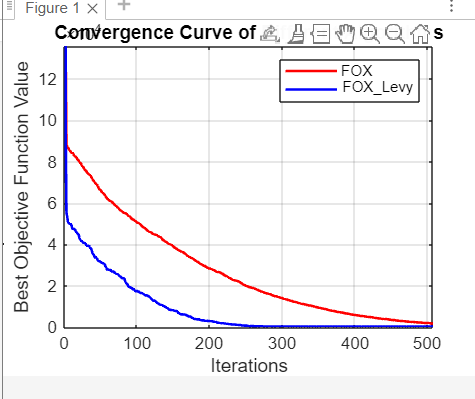
\includegraphics[width=0.5\linewidth]{Screenshot 2024-04-08 012525.png}
    \caption{CEC2017 F3 function}
    \label{fig:cec2017-f3}
\end{figure}

\begin{figure}[h!]
    \centering
    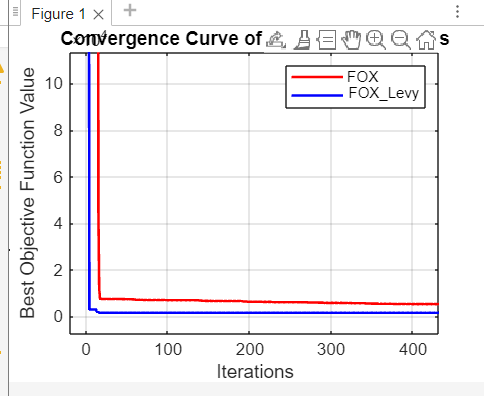
\includegraphics[width=0.5\linewidth]{Screenshot 2024-04-08 012758.png}
    \caption{CEC2017 F15 function}
    \label{fig:cec2017-f15}
\end{figure}

\begin{figure}[h!]
    \centering
    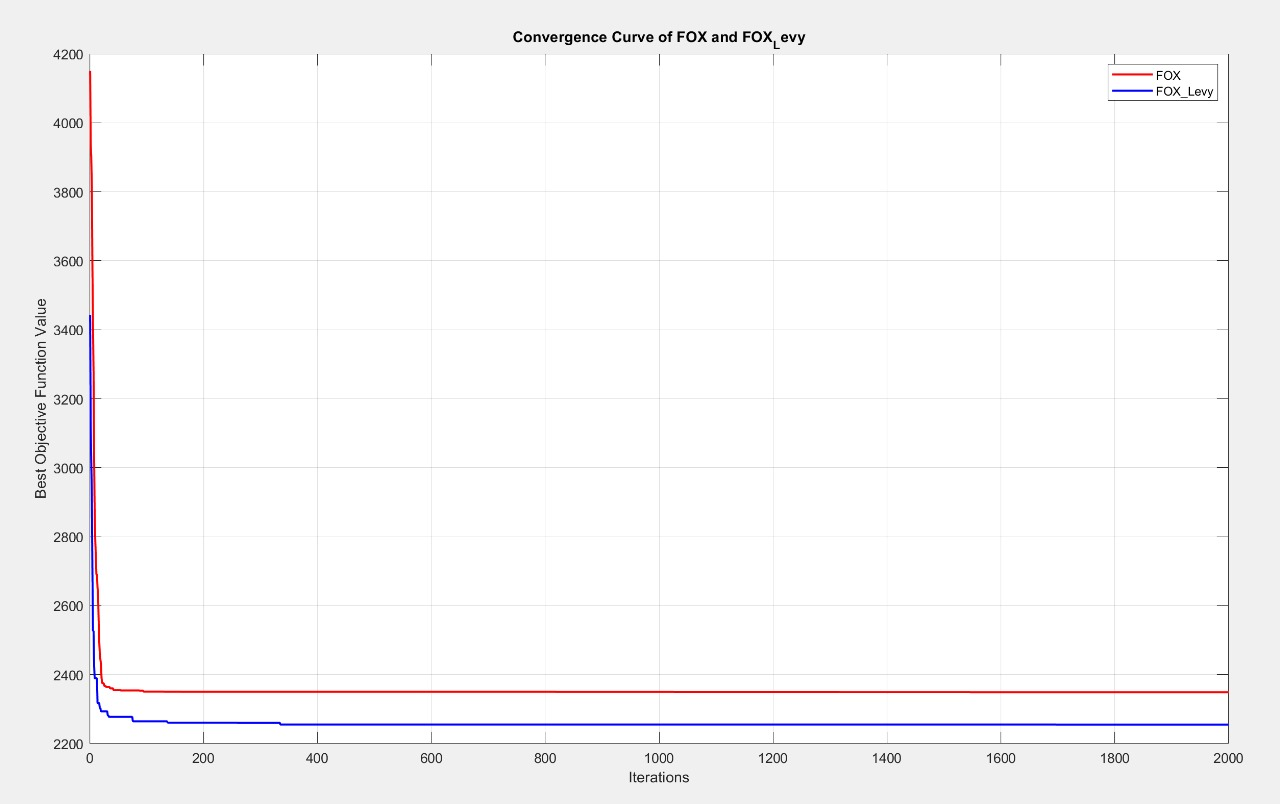
\includegraphics[width=0.5\linewidth]{WhatsApp Image 2024-04-08 at 1.36.47 AM.jpeg}
    \caption{CEC2014 F11 function}
    \label{fig:enter-label}
\end{figure}

\begin{figure}[h!]
        \centering
        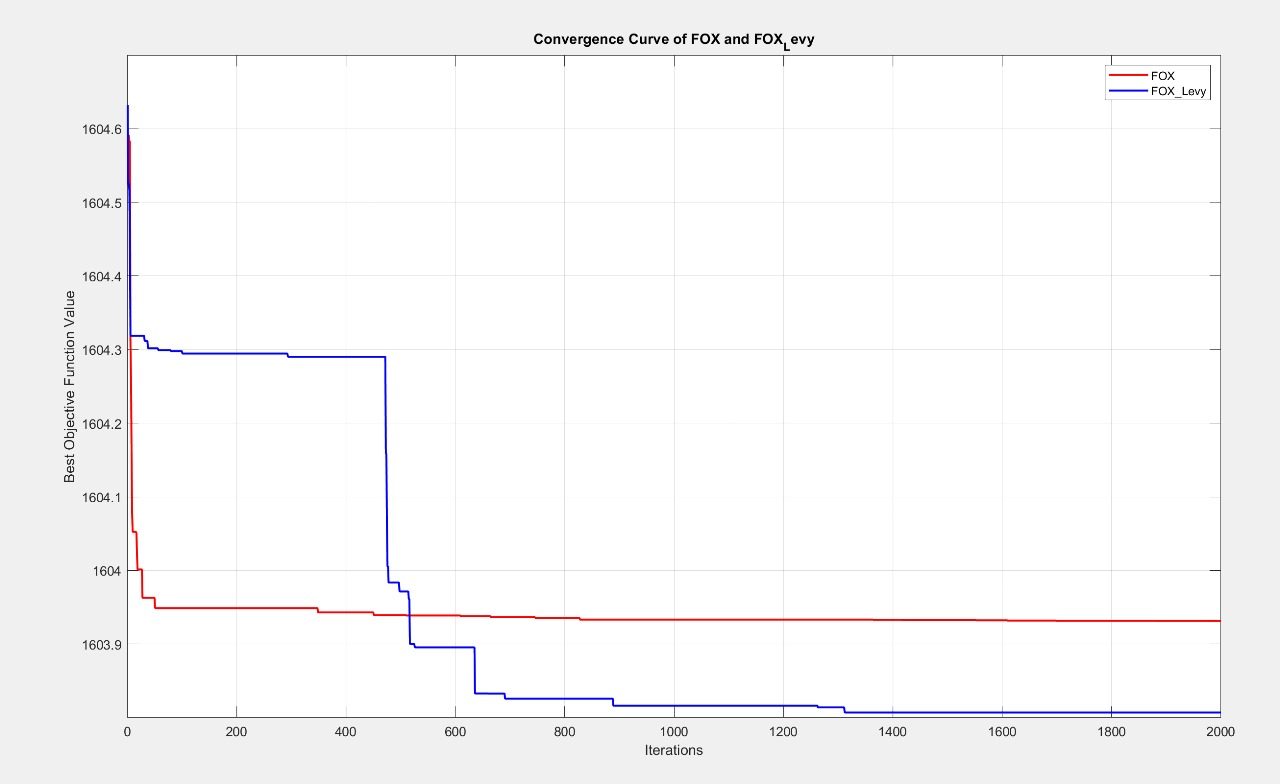
\includegraphics[width=0.5\linewidth]{WhatsApp Image 2024-04-08 at 1.55.29 AM.jpeg}
        \caption{CEC2014 F16 function}
        \label{fig:enter-label}
\end{figure}
    
\newpage
\def\labelenumi{\arabic{enumi}.}
\item
\vspace{5mm}
  \textbf{6.4 Engineering Problems}

\def\labelenumi{\arabic{enumi}.}
\item
\vspace{0.5mm}
  \textbf{6.4.1 Solving a pressure vessel design problem}
\\
The pressure vessel design problem is a fundamental challenge in engineering, frequently tackled by researchers using various optimization algorithms. The objective of this problem is to find the optimal solution for three critical aspects of a cylindrical pressure vessel: material selection, welding considerations, and forming processes. Optimization in this context typically revolves around four key variables: the shell thickness (\(T_{\text{\textit{s}}}\)), inner radius \((R)\), the length of the cylindrical section excluding the head \((L)\), and the head thickness (\(T_{\text{\textit{h}}}\)).

\begin{figure}[htbp]
    \centering
    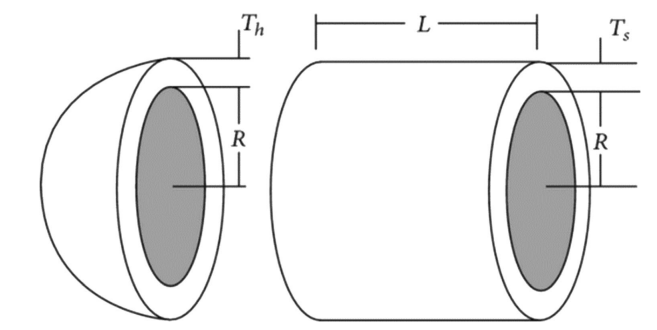
\includegraphics[width=0.8\textwidth]{pressure_vessel.png}
    \caption{Pressure Vessel Design Problem}
    \label{fig:pressure_vessel}
\end{figure}

Optimizing these variables is crucial for ensuring the pressure vessel's efficiency, safety, and cost-effectiveness. The selection of appropriate materials, welding techniques, and forming processes directly impacts the vessel's performance and longevity.

Researchers employ optimization algorithms to search for the best combination of these variables that meet specified requirements and constraints. These algorithms aim to minimize factors such as weight, cost, or material usage while adhering to standards and regulations governing pressure vessel design.
The following shows the problem equation and constraints.
\\
\begin{align*}
n &= 1, 2, 3, 4 \\
\vec{x} &= [x_1 x_2 x_3 x_4]^T = [T_s \quad T_h \quad R \quad L] \\
f(\vec{x}) &= 0.6224x_1x_3x_4 + 1.7781x_2x_3^2 + 3.1661x_1^2x_4 + 19.84x_1^2x_3 \tag{16}
\end{align*}

The variable limits are \(0 \leq x_1 \leq 99\), \(0 \leq x_2 \leq 99\), \(10 \leq x_3 \leq 200\), and \(10 \leq x_4 \leq 200\).

\begin{align*}
\tag{17}
g_1(\vec{x}) &= -x_1 + 0.0193x_3 \phantom{{} \leq 0} &  \\
\tag{18}
g_2(\vec{x}) &= -x_3 + 0.00954x_3 \phantom{{} \leq 0}  \\
\tag{19}
g_3(\vec{x}) &= -\pi x_2^3 x_4 - \frac{4}{3} \pi x_3^3 + 1.296 \times 10^6 \phantom{{} \leq 0} & \\
\tag{20}
g_4(\vec{x}) &= x_4 + 240 \phantom{{} \leq 0} 
\end{align*}


Among the optimization algorithms used for solving the pressure vessel design problem, Fox-inspired optimization algorithm and FOX Levy algorithm have demonstrated their effectiveness. By leveraging principles inspired by the behavior of foxes and incorporating Levy flight for enhanced exploration, these algorithms seek to efficiently navigate the complex solution space and converge towards optimal solutions.

Empirical studies and comparative analyses have shown that Levy Fox Algorithm often outperforms FOX in terms of convergence speed and solution quality for the pressure vessel design problem. By integrating Levy flight, FOX Levy exhibits improved exploration capabilities, enabling it to effectively explore and exploit the solution space, resulting in superior optimization outcomes compared to its predecessor FOX.

Therefore, for the pressure vessel design problem, utilizing the Levy Fox algorithm can lead to better results in terms of finding optimal solutions that meet the desired performance criteria while minimizing material usage and production costs.

\begin{table}[htbp]
\centering
\caption{Solving the Pressure Vessel Design Problem}
\vspace{1mm}
\label{tab:results}
\begin{tabular}{cccc}
\toprule
Iteration & FOX Value & FOX\_Levy Value \\
\midrule
1 & 12641.3679 & 6150.6786 \\
2 & 12877.5698 & 6100.6678 \\
3 & 15145.4906 & 6070.75 \\
4 & 6748.5045 & 7312.1903 \\
5 & 9047.6277 & 6142.2232 \\
6 & 6771.0094 & 6156.3137 \\
7 & 15348.982 & 6124.2345 \\
8 & 8558.245 & 6115.9069 \\
9 & 26694.8222 & 6416.6655 \\
10 & 10844.3545 & 6320.9083 \\
11 & 24925.6843 & 6093.8723 \\
12 & 6636.3632 & 6109.6551 \\
13 & 6317.2107 & 6437.2037 \\
14 & 18274.911 & 7051.9502 \\
15 & 13993.6494 & 6639.786 \\
16 & 9606.5879 & 6068.3024 \\
17 & 10422.2685 & 6321.8728 \\
18 & 17629.6065 & 6420.1905 \\
19 & 19650.3441 & 6095.5885 \\
20 & 30657.1377 & 6094.8735 \\
21 & 7167.2236 & 6317.0347 \\
22 & 10865.5452 & 6124.6352 \\
23 & 6238.6726 & 7309.122 \\
24 & 10473.8224 & 6126.4948 \\
25 & 12296.5508 & 6073.2574 \\
26 & 13847.6922 & 7050.1238 \\
27 & 9984.9896 & 6095.9023 \\
28 & 7337.0998 & 6076.1677 \\
29 & 6671.3945 & 6073.3758 \\
30 & 14887.1596 & 6318.2438 \\
31 & 17145.2044 & 6091.2716 \\
32 & 16398.6585 & 6101.7659 \\
33 & 8700.2457 & 6334.3122 \\
34 & 6506.0432 & 7306.7777 \\
35 & 8585.7865 & 6837.3074 \\
36 & 9443.9406 & 6424.1904 \\
37 & 7518.4132 & 6328.8611 \\
38 & 8389.642 & 6103.3602 \\
39 & 14786.3553 & 6639.4321 \\
40 & 11395.4068 & 6827.1315 \\
41 & 15343.2741 & 7048.5885 \\
42 & 12621.5802 & 6127.8585 \\
43 & 11247.2393 & 7310.4517 \\
44 & 17592.7345 & 6419.6091 \\
45 & 17205.9339 & 6118.8413 \\
46 & 10480.3975 & 6143.3261 \\
47 & 8480.2532 & 6099.076 \\
48 & 10147.9923 & 6070.9077 \\
49 & 25284.7683 & 6099.3257 \\
50 & 7603.6584 & 6647.6825 \\
\midrule
Average score & 12548.7883 & 6377.7654 \\
\bottomrule
\end{tabular}
\end{table}

\newpage
\def\labelenumi{\arabic{enumi}.}
\item
\vspace{5mm}
\textbf{6.4.2 Piston Lever}

The main objective is to locate the piston components, \( H \), \( B \), \( D \), and \( X \) by minimizing the oil volume when the lever of the piston is lifted up from \( 0^\circ \) to \( 45^\circ \) as shown below. 

\begin{figure}[htbp]
    \centering
    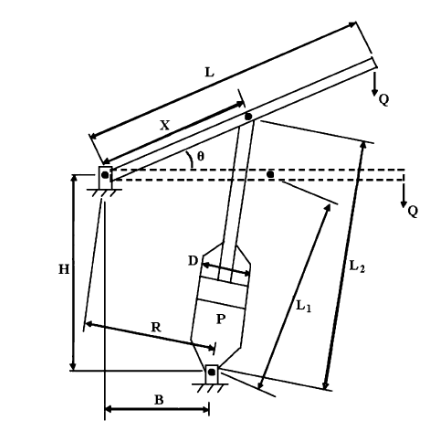
\includegraphics[width=0.6\textwidth]{piston_lever.png}
    \caption{Piston Problem}
    \label{fig:piston}
\end{figure}

The objective function of the problem is given as follows:
\[
\text{Minimize: } f(H, B, D, X) = \frac{1}{4} \pi D^2 (L_2 - L_1) \tag{21}
\]
Subject to:
\begin{align}
g_1 &= QL \cos{h} - RF \leq 0 \quad \text{at } h = 45^\circ  \tag{22} \\
g_2 &= Q(L - X) - M_{\text{max}} \leq 0 \tag{23} \\
g_3 &= 1.2(L_2 - L_1) - L_1 \leq 0 \tag{24} \\
g_4 &= \frac{D}{2} - B \leq 0 \tag{25}
\end{align}
where:
\begin{align}
R &= \frac{-X(X\sin{h} + H) + H(B - X\cos{h})}{\sqrt{(X - B)^2 + H^2}} \tag{26} \\
F &= \frac{1}{4} \pi PD^2 \tag{27} \\
L_1 &= \sqrt{(X - B)^2 + H^2} \tag{28} \\
L_2 &= \sqrt{(X \sin{45^\circ} + H)^2 + (B - X \cos{45^\circ})^2} \tag{29}
\end{align}


where the payload is \( P = 10,000 \) lbs, the lever is \( L = 240 \) in, the maximum allowable bending moment of the lever is \( M_{\text{max}} = 1.8 \times 10^6 \) lbs in, and the oil pressure is given as 1,500 psi. A number of inequality constraints are imposed. Force equilibrium, maximum bending moment of the lever, minimum piston stroke, and geometrical conditions are considered. 

The best solutions obtained are presented in Table 5.
\begin{table}[htbp]
\centering
\caption{Piston Lever Problem}
\label{tab:fox_values}
\begin{tabular}{ccc}
\toprule
Iteration & FOX\_eng & FOX\_Levy\_eng \\
\midrule
1  &  468.9598 & 474.8621 \\
2  &  2230.5645 & 780.9825 \\
3  &  1794.2828 & 343.5522 \\
4  &  1175.7539 & 290.2607 \\
5  &  627.8898 & 869.4785 \\
6  &  1935.5974 & 389.7799 \\
7  &  916.2755 & 265.8606 \\
8  &  701.6062 & 214.4843 \\
9  &  407.0287 & 248.1595 \\
10 &  751.3676 & 377.6707 \\
11 &  538.4485 & 497.6457 \\
12 &  421.8348 & 389.8757 \\
13 &  929.3762 & 508.2206 \\
14 &  417.4529 & 488.127 \\
15 &  1215.5964 & 440.5653 \\
16 &  1795.6416 & 680.9534 \\
17 &  266.4139 & 416.1447 \\
18 &  403.5552 & 219.7112 \\
19 &  354.483 & 291.2886 \\
20 &  503.6342 & 389.7389 \\
21 &  456.3015 & 585.3676 \\
22 &  469.577 & 779.8782 \\
23 &  203.9985 & 226.9539 \\
24 &  1102.5352 & 283.5069 \\
25 &  1222.8863 & 579.8735 \\
26 &  607.8286 & 420.884 \\
27 &  352.3306 & 221.0786 \\
28 &  1351.6575 & 540.1091 \\
29 &  951.4713 & 304.9573 \\
30 &  403.5566 & 279.5254 \\
31 &  656.484 & 8.9988 \\
32 &  994.7325 & 239.3712 \\
33 &  277.4978 & 316.869 \\
34 &  2399.2491 & 9.0773 \\
35 &  710.2451 & 459.9903 \\
36 &  1037.7391 & 330.4374 \\
37 &  1529.8702 & 248.0448 \\
38 &  498.6523 & 486.6814 \\
39 &  690.8866 & 769.5511 \\
40 &  764.7107 & 400.7263 \\
41 &  425.0389 & 235.6146 \\
42 &  374.4764 & 302.5955 \\
43 &  231.3713 & 355.6607 \\
44 &  235.6261 & 193.3104 \\
45 &  1033.0601 & 432.4773 \\
46 &  1049.815 & 338.8545 \\
47 &  771.6448 & 341.593 \\
48 &  624.8739 & 187.9267 \\
49 &  708.0181 & 459.6783 \\
50 &  1264.6645 & 321.7938 \\
\midrule
Average & 825.1313 & 384.775 \\
\bottomrule
\end{tabular}
\end{table}

\newpage
\def\labelenumi{\arabic{enumi}.}
\item
\vspace{5mm}
\textbf{6.4.3 Corrugated bulkhead design}\\\\
The engineering problem of corrugated bulkhead design involves designing a bulkhead structure typically used in various industries such as automotive, aerospace, and construction. A bulkhead is a structural partition that divides a space into compartments or sections, providing strength, stability, and support to the overall structure.

\begin{figure}[htbp]
    \centering
    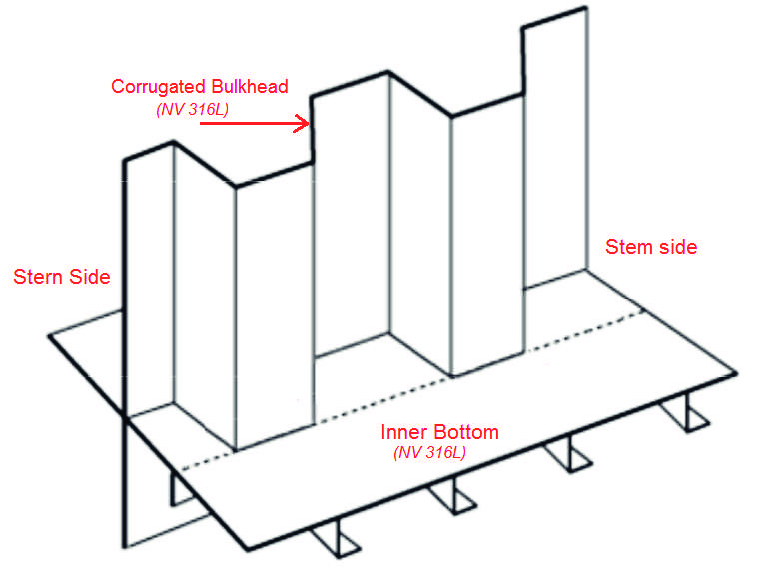
\includegraphics[width=0.6\textwidth]{bulkhead.png}
    \caption{Corrugated Bulkhead Design Problem}
    \label{fig:bulkhead}
\end{figure}

In the context of corrugated bulkhead design, the objective is to optimize the design parameters to achieve certain performance criteria while meeting specific constraints. This can include minimizing weight, maximizing strength, improving stability, reducing manufacturing costs, or enhancing other performance metrics.

The design variables for a corrugated bulkhead may include parameters such as the thickness of the material, the shape and size of the corrugations, the material properties, and the overall dimensions of the bulkhead. Constraints may arise from factors such as load-bearing requirements, space limitations, manufacturing capabilities, and regulatory standards.

The Levy fox algorithm is a metaheuristic optimization technique that can be applied to solve engineering optimization problems like corrugated bulkhead design. Levy fox algorithm optimizes the design variables iteratively, gradually improving the solution over multiple generations.

By applying the Levy fox algorithm to the corrugated bulkhead design problem, engineers can explore a wide range of design possibilities, identify optimal solutions, and efficiently navigate the design space to find high-quality designs. Compared to traditional optimization methods, Levy fox offers advantages such as faster convergence, better exploration of the design space, and robustness to noise and uncertainty.

\begin{table}[htbp]
\centering
\caption{Corrugated Bulkhead Design Problem}
\label{tab:fox_results}
\begin{tabular}{cccc}
\toprule
Iteration & FOX & FOX\_Levy & \\
\midrule
1 & 10.5023 & 6.9169 \\
2 & 7.6367 & 8.3429 \\
3 & 10.0936 & 6.9185 \\
4 & 9.1846 & 6.8814 \\
5 & 7.1097 & 7.401 \\
6 & 8.2783 & 7.0067 \\
7 & 7.3624 & 7.2062 \\
8 & 7.5956 & 7.2485 \\
9 & 8.1276 & 7.7443 \\
10 & 8.8185 & 6.9639 \\
11 & 8.3927 & 7.7596 \\
12 & 6.8607 & 7.0691 \\
13 & 7.5963 & 7.1403 \\
14 & 8.5517 & 7.1264 \\
15 & 8.5316 & 8.415 \\
16 & 8.4369 & 7.1364 \\
17 & 7.1316 & 7.3226 \\
18 & 8.6802 & 6.8988 \\
19 & 8.2371 & 7.7902 \\
20 & 8.5536 & 7.2302 \\
21 & 8.3644 & 7.9828 \\
22 & 9.149 & 8.1008 \\
23 & 10.0237 & 7.5441 \\
24 & 8.3844 & 7.0713 \\
25 & 8.0709 & 7.6164 \\
26 & 8.5294 & 7.2174 \\
27 & 8.0496 & 7.1599 \\
28 & 9.214 & 7.6291 \\
29 & 8.6568 & 8.034 \\
30 & 7.7919 & 7.164 \\
31 & 9.2603 & 6.9875 \\
32 & 8.3429 & 6.9177 \\
33 & 8.8606 & 7.0234 \\
34 & 9.0851 & 7.9971 \\
35 & 7.9749 & 7.9017 \\
36 & 7.6643 & 7.7402 \\
37 & 8.1047 & 6.9548 \\
38 & 8.375 & 7.0398 \\
39 & 8.2286 & 7.8399 \\
40 & 9.845 & 7.0184 \\
41 & 9.2729 & 7.6292 \\
42 & 7.3231 & 8.2806 \\
43 & 8.5885 & 7.2126 \\
44 & 7.7916 & 6.9483 \\
45 & 7.0829 & 7.4088 \\
46 & 8.6814 & 6.9253 \\
47 & 7.3432 & 7.5755 \\
48 & 8.2596 & 7.2447 \\
49 & 7.4372 & 7.3571 \\
50 & 8.0322 & 7.0797 \\
\midrule
Average & 8.3494 & 7.3824 \\
\bottomrule
\end{tabular}
\end{table}

\newpage
\def\labelenumi{\arabic{enumi}.}
\item
\vspace{5mm}
\textbf{6.4.4 Minimize I-beam vertical deflection}

The problem of minimizing I-beam vertical deflection is a structural engineering optimization problem commonly encountered in civil and mechanical engineering fields. In this problem, the goal is to design an I-beam structure that can withstand a given load while minimizing the vertical deflection of the beam. Vertical deflection refers to the amount of bending or sagging that occurs in the beam when subjected to a load.

\begin{figure}[htbp]
    \centering
    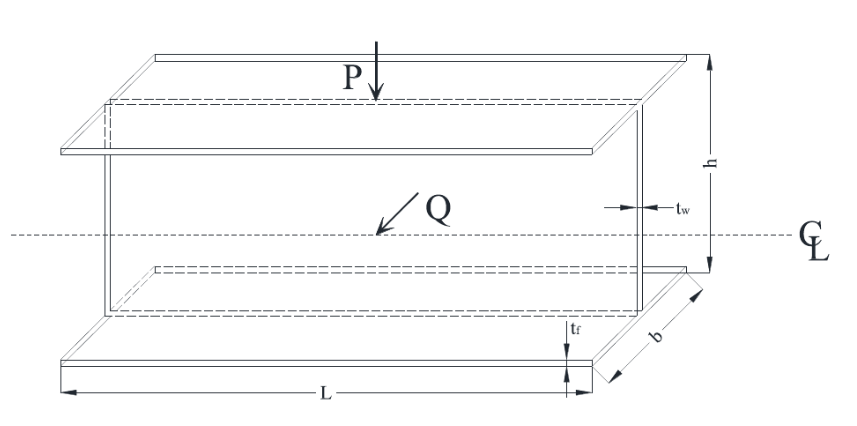
\includegraphics[width=0.6\textwidth]{beam.png}
    \caption{Minimization of I beam vertical deflection}
\end{figure}

The objective of this optimization problem is to find the dimensions of the I-beam (such as the width, height, and thickness of the flanges and web) that minimize the vertical deflection while satisfying constraints on factors such as material strength, safety factors, and geometric limitations.

The vertical deflection of an I-beam depends on various factors, including the material properties of the beam (such as modulus of elasticity and moment of inertia), the magnitude and distribution of the applied load, and the dimensions of the beam itself. The optimization problem involves finding the optimal combination of beam dimensions that minimize the vertical deflection while ensuring that the beam remains structurally sound and meets design requirements.

By applying the Levy and Fox algorithm to the I-beam vertical deflection minimization problem, we can obtain optimized beam dimensions that achieve the desired performance criteria. The algorithm iteratively explores the solution space, adjusting the beam dimensions to minimize the vertical deflection while satisfying all constraints. The resulting beam design represents an optimal balance between structural integrity, material efficiency, and performance compared to the fox algorithm. The results obtained are presented in table 7.

\begin{table}[htbp]
\centering
\caption{Minimize I-beam vertical deflection}
\label{tab:fox_results}
\begin{tabular}{cccc}
\toprule
Iteration & FOX & FOX\_Levy & \\
\midrule
1 & 0.015094 & 0.013414 \\
2 & 0.085443 & 0.013454 \\
3 & 0.021192 & 0.013504 \\
4 & 0.01369 & 0.013259 \\
5 & 0.017802 & 0.013077 \\
6 & 0.013574 & 0.013316 \\
7 & 0.023668 & 0.013083 \\
8 & 0.018008 & 0.013208 \\
9 & 0.014242 & 0.013094 \\
10 & 0.013533 & 0.013229 \\
11 & 0.030265 & 0.013462 \\
12 & 0.016603 & 0.01325 \\
13 & 0.021594 & 0.013144 \\
14 & 0.021374 & 0.013283 \\
15 & 0.0229 & 0.013214 \\
16 & 0.013528 & 0.013191 \\
17 & 0.16858 & 0.013449 \\
18 & 0.014177 & 0.013116 \\
19 & 0.091301 & 0.01308 \\
20 & 0.033586 & 0.013571 \\
21 & 0.016429 & 0.013302 \\
22 & 0.01327 & 0.013281 \\
23 & 0.013377 & 0.013417 \\
24 & 0.013379 & 0.013097 \\
25 & 0.013241 & 0.013112 \\
26 & 0.01522 & 0.013382 \\
27 & 0.20739 & 0.013082 \\
28 & 0.013293 & 0.013459 \\
29 & 0.024302 & 0.013184 \\
30 & 0.023673 & 0.013081 \\
31 & 0.05274 & 0.013462 \\
32 & 0.019337 & 0.013221 \\
33 & 0.013479 & 0.013088 \\
34 & 0.013717 & 0.013125 \\
35 & 0.15601 & 0.013194 \\
36 & 0.0133 & 0.013165 \\
37 & 0.088685 & 0.013116 \\
38 & 0.029383 & 0.013108 \\
39 & 0.014496 & 0.013114 \\
40 & 0.013724 & 0.013387 \\
41 & 0.015753 & 0.013232 \\
42 & 0.023742 & 0.013389 \\
43 & 0.12526 & 0.013195 \\
44 & 0.10945 & 0.013199 \\
45 & 0.013795 & 0.013282 \\
46 & 0.013832 & 0.013303 \\
47 & 0.013221 & 0.013381 \\
48 & 0.223 & 0.013085 \\
49 & 0.021512 & 0.013283 \\
50 & 0.017634 & 0.013312 \\
\midrule
Average & 8.3494 & 7.3824 \\
\bottomrule
\end{tabular}
\end{table}

\newpage
\textbf{7. Conclusion}

\vspace{1mm}

In conclusion, the incorporation of Levy flight into the FOX algorithm significantly enhances its exploration capabilities while complementing the exploitation capabilities already inherent in FOX. LLFOA (Levy Flight ased Fox Optimization Algorithm) enables efficient exploration of diverse regions within the search space, leading to improved convergence rates and the discovery of high-quality solutions across various benchmark functions. This synergy between exploration and exploitation is crucial for tackling complex optimization landscapes effectively.

Moving forward, there are several promising avenues for further research and development. Fine-tuning the parameters of Levy flight within LLFOA can optimize its exploration-exploitation balance for specific problem domains, potentially enhancing its performance. Additionally, exploring hybrid approaches that combine Levy flight with other search strategies or optimization techniques could lead to even greater performance improvements, particularly in dynamic or multi-objective optimization scenarios. Scalability and parallelization techniques can also be investigated to improve LLFOA's efficiency in handling large-scale optimization problems. Moreover, validating LLFOA on real-world applications across different domains can provide insights into its practical effectiveness and identify specific use cases where it excels. Finally, developing algorithmic variants or extensions of LLFOA to address specific optimization challenges, such as constrained optimization or noisy objective functions, can further broaden its applicability and robustness. These avenues represent valuable directions for advancing LLFOA and establishing it as a reliable and versatile optimization algorithm for solving a wide range of complex optimization problems.
\vspace{8mm}



\newpage


  
\end{document}